% ============================================================
%  IROS 2026 — IEEEtran Conference Template (double-column)
% ============================================================
\documentclass[conference]{IEEEtran}
\IEEEoverridecommandlockouts

% ── Packages ────────────────────────────────────────────────
\usepackage{cite}
\usepackage{amsmath,amssymb,amsfonts}
\usepackage{graphicx}
\usepackage{textcomp}
\usepackage{booktabs}
\usepackage{xcolor}
\usepackage{url}
\usepackage{float}

% ── Algorithm counter (standalone, no algorithm package) ────
\newcounter{algctr}
\renewcommand{\thealgctr}{\arabic{algctr}}

\graphicspath{{figures/}}

% ── Macros ──────────────────────────────────────────────────
\newcommand{\eg}{\textit{e.g.}}
\newcommand{\ie}{\textit{i.e.}}
\newcommand{\etal}{\textit{et al.}}
\newcommand{\rmha}{\textsc{rmha}}

% ============================================================
\begin{document}

\title{SPARC: Spatial-Aware Path Planning via Attentive Robot Communication}

% ── Authors ──────────────────────────────────────────────────
\author{
\IEEEauthorblockN{Sayang Mu, Xiangyu Wu, and Bo An$^{\dagger}$}
\IEEEauthorblockA{Nanyang Technological University, Singapore\\
Email: \{xiangyu015, sayang001, boan\}@ntu.edu.sg}
\thanks{$^{\dagger}$Corresponding author.}
}

\maketitle

% ============================================================
%  ABSTRACT
% ============================================================
\begin{abstract}
This paper addresses the problems of low communication efficiency
and insufficient cooperative optimization in Multi-Robot Path
Planning (MRPP) by proposing an efficient communication method
called Relation-enhanced Multi-Head Attention (\rmha) based on
graph attention mechanisms.
By introducing a spatial relation-enhanced multi-head attention
structure, \rmha{} organically combines the relative distance
information between robots with communication content, enabling
dynamic allocation and optimization of communication weights.
This effectively reduces communication overhead while improving
overall planning performance.
Experimental results demonstrate that \rmha{} exhibits strong
adaptability and robustness across environments with varying
obstacle densities, with particularly significant advantages in
high-density complex scenarios where its path planning success
rate substantially outperforms existing methods.
Furthermore, ablation studies confirm the critical role of
distance information in communication modeling and path
decision-making, showing that this mechanism promotes efficient
inter-robot cooperation and information sharing.
In summary, \rmha{} offers high practical value and scalability
for cooperative path planning in multi-robot systems, providing
a new perspective on agent communication and collaboration in
complex environments.
\end{abstract}

\begin{IEEEkeywords}
Multi-robot path planning, graph attention mechanism, multi-head
attention, communication optimization, cooperative decision-making
\end{IEEEkeywords}

% ============================================================
%  1  INTRODUCTION
% ============================================================
\section{Introduction}

Multi-Robot Path Planning (MRPP) is a core problem in artificial
intelligence and robotics, aiming to design collision-free paths
for multiple robots to navigate from their respective starting
positions to goal positions in a known environment~\cite{wang2023scrimp}.
In this paper, the terms \emph{agent} and \emph{robot} are used
interchangeably.
In the standard MRPP formulation, a graph structure represents the
robots' workspace together with sets of start and goal
vertices.
At each time step, a robot may either stay at its current vertex
or move to an adjacent one~\cite{li2021lifelong}.
A solution to an MRPP instance is a set of paths—one per robot—that
are free of both vertex and edge collisions.
Finding such a solution is known to be NP-hard.

An MRPP instance is defined by a graph, a set of robots, and their
respective start–goal pairs.
The problem can be viewed as a planning challenge whose objective
is to find a collision-free path set (the \emph{solution}) for a
given instance.
An MRPP \emph{algorithm} (or \emph{solver}) refers to the method
used to compute such a solution.

MRPP has broad applications in intelligent warehousing
systems~\cite{zhang2023warehouse}, urban traffic
networks~\cite{dresner2008multiagent}, autonomous
vehicles, and electronic games, among
others~\cite{ma2022graph}.
As a foundational task in building physical multi-robot systems,
MRPP plays a pivotal role in the design phase and its importance
is expected to grow as demand for cooperative and competitive
multi-robot scenarios increases.

%\begin{figure}[t]
%\centering
%
\includegraphics[width=\columnwidth]{image}
%\caption{Application scenarios of MRPP.}
%\label{fig:app_scenarios}
%\end{figure}

In the warehouse logistics domain in particular, the rapid
expansion of e-commerce has made intelligent logistics systems
indispensable.
Autonomous Mobile Robots (AMR)~\cite{tamura2025human} are
increasingly deployed in unmanned warehouses.
For such AMR-based warehousing systems, path planning is the core
scheduling component.
However, as the number of robots and the complexity of tasks
increase, efficiently and safely planning collision-free paths
remains a critical challenge.

\subsection{Centralized Planning Methods}

Centralized approaches rely on a central controller with
complete global information to compute (near-)optimal paths.

\textbf{A* and its variants.}
A* is a classic heuristic search algorithm whose evaluation
function is $f(n)=g(n)+h(n)$.
Extensions to multi-robot settings include LRA*, which adjusts
trajectories upon detecting potential conflicts; CA*, which
introduces a three-dimensional reservation table to avoid
collisions~\cite{silver2005cooperative}; and HCA*, which
employs hierarchical abstraction to improve scalability.
However, frequent replanning in dense scenarios leads to
high computational overhead.

\textbf{Conflict-Based Search (CBS)} uses a two-level search:
the high level discovers and decomposes conflicts, while the low
level computes optimal single-robot paths under
constraints~\cite{sharon2015cbs}.
A binary constraint tree is constructed until a conflict-free
solution is found.

\textbf{ODrM*} combines decoupled and coupled strategies: each
robot initially follows its individual optimal path; upon
collision, only the conflicting robots are coupled for joint
search~\cite{ren2021subdimensional,ellis2021mapf}.
While effective as a bounded sub-optimal planner, ODrM* suffers
from exponential complexity growth when the number of agents or
environment complexity increases.

\subsection{Decentralized Learning-Based Methods}

Centralized methods struggle with real-time requirements and
scalability as the number of robots and environment size grow.
Multi-Agent Reinforcement Learning (MARL) offers an effective
alternative under partial observability: agents access only
local observations and make fast, decentralized
decisions~\cite{huang2021strategic}.

Learning-based methods typically train a policy that maps local
observations (\eg, a limited Field of View, FOV) to discrete
actions (up/down/left/right/wait) on a grid world.
Major paradigms include Imitation Learning (IL), which imitates
demonstrations from centralized solvers, and Reinforcement
Learning (RL), which maximizes expected return.
In MRPP, the problem is commonly modeled as a
Dec-POMDP~\cite{huang2021strategic}.
PRIMAL~\cite{sartoretti2019primal} integrates physical simulation
with hybrid offline--online training;
LNS2+RL~\cite{wang2025lns2rl} fuses large neighborhood search
with MARL;
Li~\etal~first introduced GNNs for MRPP, encoding FOV
interactions and supporting decentralized
decisions~\cite{li2020gnn,li2021magat}.

\subsection{Contributions}

The main contributions of this work are as follows:
\begin{enumerate}
\item We propose a \textbf{spatial relation-enhanced multi-head
      attention communication mechanism} that incorporates
      inter-robot relative distance as edge information into the
      attention weight computation, enabling communication weights
      to adapt dynamically to topological relationships and
      improving cooperative decision-making.
\item We construct an \textbf{end-to-end cooperative learning
      framework based on MAPPO}, introducing distance-constrained
      local communication and attention masking to reduce
      communication overhead while maintaining effective
      information exchange and training stability.
\item We design \textbf{communication ablation studies and
      multi-density scenario evaluations} that quantitatively
      verify the critical role of distance-relation encoding for
      success rate improvement and congestion/conflict mitigation,
      demonstrating stronger robustness in high-density
      environments.
\end{enumerate}

% ============================================================
%  2  METHOD
% ============================================================
\section{Spatial Relation-Enhanced Multi-Head Attention\\
Communication for Multi-Robot Path Planning}

\subsection{System Model and Problem Formulation}

\subsubsection{MRPP System Model}

The MRPP problem can be formally defined as a four-tuple
$\langle \mathcal{A}, G, \mathcal{O}_{\mathrm{dyn}},
\mathcal{O}_{\mathrm{static}} \rangle$, where:
$\mathcal{A}=\{A_1, A_2, \ldots, A_N\}$ is the set of $N$ robots;
$G=(V,E)$ is a graph representing the environment with vertex set
$V$ (locations) and edge set $E$ (traversable connections);
$\mathcal{O}_{\mathrm{dyn}}=\{O_1^d, \ldots, O_M^d\}$ denotes $M$
dynamic obstacles whose positions change over time; and
$\mathcal{O}_{\mathrm{static}}=\{O_1^s, \ldots, O_K^s\}$ denotes
$K$ static obstacles.

Each robot $A_n \in \mathcal{A}$ is represented by a tuple
$\langle s_n, g_n \rangle$, where $s_n$ and $g_n$ are the start
and goal positions, respectively.
A valid MRPP solution must satisfy:

\begin{enumerate}
\item \textbf{Deadlock-free constraint:}
There exists a finite time step $T \in \mathbb{Z}^+$ such that all
robots reach their goals.
\item \textbf{Vertex collision-free constraint:}
For any two robots $A_n$ and $A_{n'}$ and any time step
$0 \le t \le T$, their positions must not coincide, nor may any
robot occupy a position held by a static or dynamic obstacle.
\item \textbf{Edge collision-free constraint:}
No two robots may simultaneously traverse the same edge in
opposite directions.
\end{enumerate}

When multiple valid solutions exist, MRPP can be cast as an
optimization problem. Common objectives include the
\emph{makespan}:
\begin{equation}\label{eq:makespan}
  M(\pi) = \max_{1 \le k \le N} |\Pi_k|,
\end{equation}
and the \emph{Sum of Costs (SOC)}:
\begin{equation}\label{eq:soc}
  \mathrm{SOC}(\pi) = \sum_{k=1}^{N} |\Pi_k|,
\end{equation}
where $|\Pi_k|$ denotes the path length of robot $k$.
These two objectives optimize the solution from the perspectives
of time and total path length, respectively.

\begin{figure}[t]
\centering
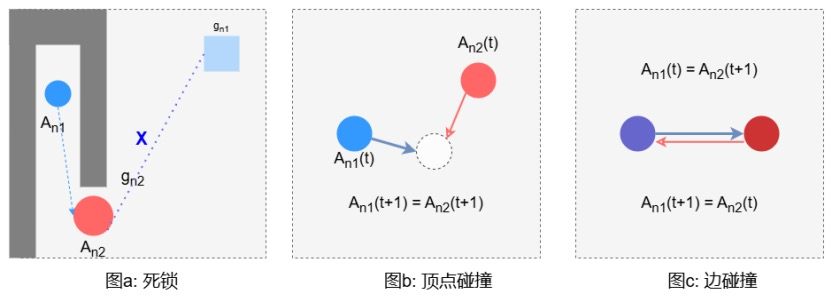
\includegraphics[width=0.85\columnwidth]{mrpp-constraints}
\caption{Illustration of MRPP constraints: vertex collisions,
edge collisions, and swap collisions must all be avoided.}
\label{fig:mrpp_constraints}
\end{figure}

\textbf{Reward design in RL-based MRPP.}
Table~\ref{tab:reward_survey} summarizes the reward mechanisms
used in representative RL-based MRPP methods.
Core elements include movement penalties and collision penalties
to constrain redundant actions and conflict risks, heuristic-based
sub-goal positive feedback to guide progressive goal achievement,
and mechanisms that suppress blocking, deadlock, and path
deviation to improve cooperation efficiency.

\begin{table*}[t]
\centering
\caption{Comparison of Reward Designs in RL-based MRPP Methods}
\label{tab:reward_survey}
\renewcommand{\arraystretch}{1.1}
\setlength{\tabcolsep}{4pt}
\footnotesize
\begin{tabular}{lc cccc cc ccc}
\toprule
\textbf{Method} & \textbf{Year}
& \textbf{Move} & \textbf{Wait$^{a}$} & \textbf{Wait$^{b}$}
& \textbf{Coll.} & \textbf{Ego-goal} & \textbf{All-goal}
& \textbf{Block} & \textbf{Oscil.} & \textbf{Deviate} \\
\midrule
PRIMAL   & 2019 & $\downarrow$ & $\downarrow$ & $\rightarrow$ & $\downarrow$ & --             & $\uparrow$   & $\downarrow$ & --           & -- \\
GNN      & 2020 & --           & --           & --            & --           & --             & --           & --           & --           & -- \\
MAPPER   & 2020 & $\downarrow$ & $\downarrow$ & $\downarrow$  & $\downarrow$ & $\uparrow$     & --           & --           & $\downarrow$ & $\downarrow$ \\
G2RL     & 2020 & $\downarrow$ & --           & --            & $\downarrow$ & --             & $\uparrow$   & --           & --           & -- \\
PRIMAL2  & 2021 & $\downarrow$ & $\downarrow$ & $\rightarrow$ & $\downarrow$ & $\uparrow$     & --           & --           & --           & -- \\
MAGAT    & 2021 & --           & --           & --            & --           & --             & --           & --           & --           & -- \\
DHC      & 2021 & $\downarrow$ & $\downarrow$ & $\rightarrow$ & $\downarrow$ & $\uparrow$     & --           & $\downarrow$ & --           & -- \\
PICO     & 2022 & $\downarrow$ & $\downarrow$ & $\rightarrow$ & $\downarrow$ & --             & $\uparrow$   & --           & --           & -- \\
DCC      & 2022 & $\downarrow$ & $\downarrow$ & $\rightarrow$ & $\downarrow$ & $\uparrow$     & --           & --           & --           & -- \\
SACHA    & 2023 & $\downarrow$ & $\downarrow$ & $\rightarrow$ & $\downarrow$ & $\uparrow$     & --           & $\downarrow$ & --           & -- \\
SCRIMP   & 2023 & $\downarrow$ & $\downarrow$ & $\rightarrow$ & $\downarrow$ & $\rightarrow$  & $\uparrow$   & --           & --           & -- \\
\bottomrule
\multicolumn{11}{l}{\scriptsize $^{a}$Not at goal.\quad $^{b}$At goal.\quad
$\downarrow$\,=\,penalty;\;$\uparrow$\,=\,reward;\;$\rightarrow$\,=\,neutral;\;--\,=\,not used.}
\end{tabular}
\end{table*}

\subsubsection{Problem Formulation}

In this work, the MRPP problem is defined by a set of robots
$\{1,\ldots,n\}$ and represented as a tuple
$\langle G, S, T \rangle$, where $G=(V,E)$ is an undirected graph,
$S=\{s_1,\ldots,s_n\}\subset V$ and
$T=\{t_1,\ldots,t_n\}\subset V$ are the start and goal positions,
respectively~\cite{chung2024review}.
Time is discretized into steps; at each step a robot may move to
an adjacent vertex or stay, provided the action does not cause a
vertex, edge, or swap collision.
The objective is to find the shortest joint collision-free path
from $S$ to $T$.

In the MARL setting, the problem is modeled as a Markov game
$\langle \mathcal{N}, \mathcal{O}, \mathcal{A}, R, P, \gamma
\rangle$, where
$\mathcal{N}=\{1,\ldots,N\}$ is the robot set;
$\mathcal{O}=\prod_{i=1}^{N}\mathcal{O}_i$ is the joint
observation space;
$\mathcal{A}=\prod_{i=1}^{N}\mathcal{A}_i$ is the joint action
space;
$R:\mathcal{O}\times\mathcal{A}\to[-R_{\max},R_{\max}]$ is the
joint reward function;
$P:\mathcal{O}\times\mathcal{A}\times\mathcal{O}\to\mathbb{R}$
is the transition probability; and
$\gamma\in(0,1)$ is the discount factor.

At each time step $t$, robot~$i$ receives observation
$o_i^t\in\mathcal{O}_i$ and selects action $a_i^t$ according to
its policy $\pi_i$.
The objective is to maximize the cumulative discounted reward:
\begin{equation}\label{eq:return}
  R_\gamma = \sum_{t=0}^{\infty} \gamma^t\, R(o^t, a^t).
\end{equation}

% ── 2.2 ────────────────────────────────────────────────────
\subsection{Spatial Relation-Enhanced Multi-Head Attention
Communication Algorithm}

\subsubsection{MDP Modeling for MRPP}

MRPP can be modeled as a Markov Game (MG), an extension of the
Markov Decision Process (MDP) to multi-agent
settings~\cite{huang2021strategic}.
An MDP is defined by a five-tuple $\langle S, A, T, R, \gamma
\rangle$.
In an MG with $N$ robots, the action space extends to the joint
space $\mathcal{A}^{1\ldots N}=\mathcal{A}_1\times\cdots\times
\mathcal{A}_N$, and the reward function becomes a set
$\mathcal{R}=\{R_1,\ldots,R_N\}$ with
$R_n:S\times\mathcal{A}_n\to\mathbb{R}$.
Under partial observability, the model becomes a Partially
Observable Markov Game
(POMG)~\cite{ma2021distributed}, where each robot observes only
a local view $o_n\in\mathcal{O}_n$.
Alternatively, a Dec-POMDP formulation can be used, represented as
$\langle \mathcal{O}, S, \mathcal{A}, T, R, \phi, \gamma
\rangle$, where $\phi$ denotes the conditional observation
distribution~\cite{guan2022abmapper}.

\begin{figure}[t]
\centering
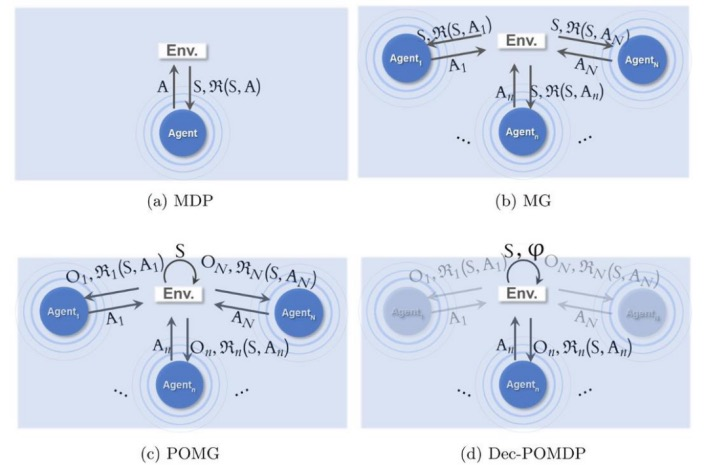
\includegraphics[width=0.85\columnwidth]{marl-modeling}
\caption{MARL modeling paradigms for MRPP: MG, POMG, and
Dec-POMDP.}
\label{fig:marl_modeling}
\end{figure}

To cast MRPP as an RL problem, we construct a discrete
two-dimensional grid world.
Robots, goals, and obstacles each occupy one cell.
At the start of each episode, $n$ unique start and goal positions
are randomly assigned within the same connected region.
Robots move simultaneously and collisions are checked on the joint
action vector.
Each robot's FOV is limited to $3\times 3$.

\textbf{State space $\mathcal{S}$:}
Each robot's observation consists of two parts.
The first comprises eight binary matrices: four heuristic maps
(one per movement direction, with a cell marked~1 iff executing
that action brings the robot closer to its goal) and four maps
encoding nearby obstacles, other robots' positions, the robot's
own goal, and projected goal positions of observable peers.
The second is a 7-dimensional vector containing the normalized
distance to the goal ($d_x$, $d_y$, $d$), the extrinsic reward
$r_{t-1}^e$, the intrinsic reward $r_{t-1}^i$, the minimum
Euclidean distance $d_{\min}^{t-1}$ to positions stored in a
short-term memory buffer, and the previous action $a_{t-1}$.

\textbf{Action space $\mathcal{A}$:}
$\mathcal{A}=\{\text{Up}, \text{Down}, \text{Left}, \text{Right},
\text{Stay}\}$.
Actions are feasible only if they do not cause vertex, edge, or
swap collisions.

\textbf{Reward $R$:}
The reward structure is summarized in Table~\ref{tab:reward}.
Robots that have not yet reached their goals receive a per-step
penalty to encourage faster completion.
An episode terminates when all robots reach their goals or a
maximum of 256 time steps is reached.
Communication messages are subject to a one-step delay and are not
blocked by obstacles.

\begin{table}[t]
\centering
\caption{Reward Settings}
\label{tab:reward}
\begin{tabular}{lc}
\toprule
\textbf{Action} & \textbf{Reward} \\
\midrule
Move (up/down/left/right) & $-0.3$ \\
Stay (at goal / off goal) & $0.0$ / $-0.3$ \\
Collision & $-2.0$ \\
Blocking & $-1.0$ \\
\bottomrule
\end{tabular}
\end{table}

% ── 2.2.2 RMHA ─────────────────────────────────────────────
\subsubsection{The RMHA Communication Mechanism}

To design an efficient communication paradigm for MARL-based
MRPP, we adopt a communication
Transformer~\cite{wang2025transformer,xiong2025ropt,lee2024mission}
inspired by the graph modeling paradigm.
We apply the Transformer Encoder architecture to map the input
observation sequence $(o_1,\ldots,o_N)$ to the output action
sequence $(a_1,\ldots,a_N)$.
Each encoder block consists of a spatial relation-enhanced
attention mechanism, a multi-layer perceptron
(MLP)~\cite{aina2025mlp,wang2025mlp,ouaret2025mlp}, and residual
connections.

In the standard multi-head attention, the attention score between
elements $o_i$ and $o_j$ is computed as the dot product of their
query and key vectors:
\begin{equation}\label{eq:vanilla_attn}
  s_{ij} = f(o_i, o_j) = o_i\, W_q^\top W_k\, o_j,
\end{equation}
which can be viewed as implicit edge information associated with
the directed edge $e_{j\to i}$.

We propose a \textbf{Spatial Relation-Enhanced Multi-Head
Attention} (\rmha) mechanism that explicitly incorporates
inter-robot spatial relationships into the attention
computation~\cite{xiao2025collaborative,chen2025predicting,chen2023transportation}.
Specifically, the Manhattan distance between robots is embedded
into a high-dimensional vector space and combined with local
observations to jointly compute attention scores:
\begin{equation}\label{eq:rmha_attn}
  s_{ij} = g(o_i, o_j, d_{i\to j}, d_{j\to i})
         = (o_i + d_{i\to j})\, W_q^\top W_k\, (o_j + d_{j\to i}),
\end{equation}
where $d_{*\to *}$ denotes the embedding vector of the Manhattan
distance between the corresponding robots.
The encoded observations $(o_1,\ldots,o_N)$ thus capture not only
individual robot information but also higher-level spatial
relationships through communication.

\textbf{Communication range constraint.}
In practice, each robot can only communicate with a limited number
of peers due to bandwidth and medium-access contention.
To model this, each robot communicates only with those within a
specified radius $R$:
\begin{equation}\label{eq:comm_neighbor}
  \mathcal{N}_i(t) = \{j \mid d_{ij}(t) \le R,\; j \ne i\},
\end{equation}
where $d_{ij}(t)$ is the distance between robots $i$ and $j$ at
time $t$.
An adjacency-based mask is applied to the attention scores:
\begin{equation}\label{eq:mask}
  \tilde{s}_{ij} =
  \begin{cases}
    s_{ij},   & \text{if } e_{j\to i} = 1, \\
    -\infty,  & \text{if } e_{j\to i} = 0,
  \end{cases}
\end{equation}
ensuring that only information from connected robots is accessible.

\begin{figure}[t]
\centering
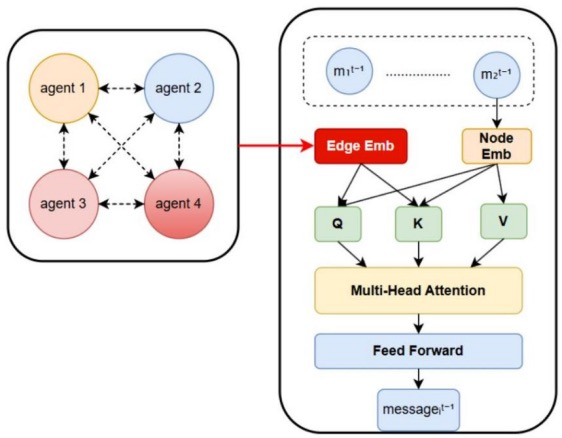
\includegraphics[width=\columnwidth]{rmha-module}
\caption{Architecture of the \rmha{} communication module.}
\label{fig:rmha_arch}
\end{figure}

% ── 2.2.3 Integration with MAPPO ───────────────────────────
\subsubsection{Integration with MAPPO}

We adopt Multi-Agent Proximal Policy Optimization
(MAPPO)~\cite{zhou2025mappo,zhang2025mappo,ding2025mappo}
as the base training framework.
The neural network model integrates three components
(Fig.~\ref{fig:rmha_net}):

\textbf{(1) Multi-modal observation encoder.}
A backbone of seven convolutional layers and two max-pooling
layers extracts spatial features, followed by three fully
connected layers for dimensionality reduction.
For robot $i$ at time $t$, the local observation
$o_i^t \in \mathbb{R}^{4\times m\times m}$ is processed by:
\begin{equation}\label{eq:conv}
  \hat{o}_i^t = \mathrm{Conv}_2\!\bigl(\mathrm{MP}\bigl(
    \mathrm{Conv}_1(o_i^t)\bigr)\bigr),
\end{equation}
\begin{equation}\label{eq:fc_concat}
  \bar{o}_i^t = \mathrm{FC}_1\!\bigl(\mathrm{concat}\bigl(
    \hat{o}_i^t,\; \mathrm{FC}_0(v_i^t)\bigr)\bigr),
\end{equation}
where $v_i^t$ is the 7-dimensional state vector.
Temporal fusion is achieved via an LSTM unit:
\begin{equation}\label{eq:lstm}
  h_i^t = \mathrm{LSTM}(\bar{o}_i^t, h_i^{t-1}).
\end{equation}

\textbf{(2) Distributed communication module.}
Built on the Transformer encoder, this module deeply fuses the
quantized Manhattan distance representation with attention weight
computation.
For a group of $n$ robots, the queries, keys, and values are:
\begin{align}
  Q &= W_q\bigl(M^{t-1} + W_1 \cdot \mathrm{Distance}\bigr),
      \label{eq:Q} \\
  K &= W_k\bigl(M^{t-1} + W_2 \cdot \mathrm{Distance}\bigr),
      \label{eq:K} \\
  V &= W_v\, M^{t-1}, \label{eq:V}
\end{align}
where $M^{t-1}\in\mathbb{R}^{n\times d}$ is the message matrix
from the previous time step, and
$W_1\cdot\mathrm{Distance}$ encodes explicit edge information.
The attention weights are computed using scaled dot-product
attention:
\begin{equation}\label{eq:attn_weight}
  \alpha_i = \mathrm{softmax}\!\left(
    \frac{q_i\, K^\top}{\sqrt{d_k}}\right).
\end{equation}
Information aggregation is performed through multi-head attention:
\begin{equation}\label{eq:head}
  \mathrm{head}_i = \alpha_i\, V,
\end{equation}
\begin{equation}\label{eq:msg}
  m_i^{t-1} = \mathrm{concat}\!\bigl(
    \mathrm{head}_i^1, \ldots, \mathrm{head}_i^h\bigr)\, W_o.
\end{equation}
Local communication is enforced via a mask matrix
$\mathcal{M}_{ij}=-\infty \cdot \mathbf{1}(\|p_i-p_j\|_2 > r)$,
where $r$ is the communication radius.

\textbf{(3) Output heads.}
The LSTM hidden state and the communication message are
concatenated and fed to four output heads that produce:
(i)~the message vector for the next time step,
(ii)~state-value estimates for extrinsic and intrinsic rewards,
(iii)~the policy distribution
$\pi_i(a^t \mid o^t)$, and
(iv)~a blocking flag indicating whether the robot obstructs
other agents' paths.

The policy is optimized using the clipped PPO objective:
\begin{equation}\label{eq:ppo}
  L_\pi(\theta) = \mathbb{E}_t\!\left[\min\!\bigl(
    r_t(\theta)\hat{A}_t,\;
    \mathrm{clip}(r_t(\theta), 1\!\pm\!\epsilon)\hat{A}_t
  \bigr)\right],
\end{equation}
where $\hat{A}_t$ is the Generalized Advantage Estimation (GAE)
and $r_t(\theta)=\pi_\theta(a_t|o_t)/\pi_{\theta_{\mathrm{old}}}
(a_t|o_t)$ is the importance sampling ratio.

\begin{figure}[t]
\centering
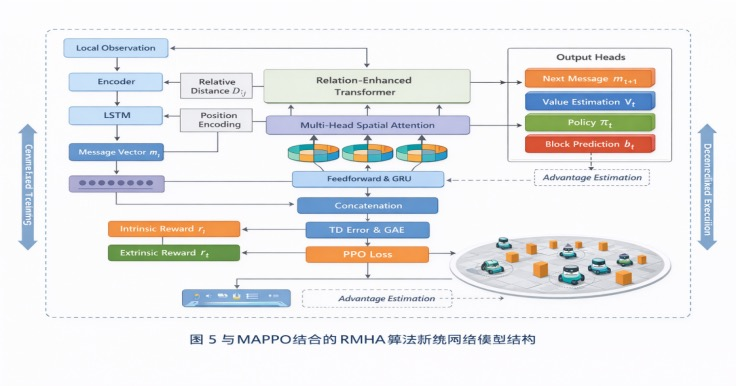
\includegraphics[width=\columnwidth]{rmha-network}
\caption{Network architecture of \rmha{} integrated with MAPPO.}
\label{fig:rmha_net}
\end{figure}

MAPPO employs Centralized Training with Decentralized Execution
(CTDE): during training, agents share environment states, actions,
and rewards to build a globally informed joint policy model; during
execution, each agent relies solely on local observations for
independent decision-making.

The complete training procedure is presented in
Algorithm~\ref{alg:rmha}.

\begin{figure}[t]
\refstepcounter{algctr}
\hrule\smallskip
\noindent\textbf{Algorithm~\thealgctr}\quad \rmha{} Training Procedure
\label{alg:rmha}\smallskip\hrule\smallskip
{\small
\noindent\textbf{Input:} Robot count $N$, episodes $K$, steps per
episode $T$, FOV size $F$, Transformer layers $L$, discount
$\gamma$, PPO clip $\epsilon$, intrinsic reward params
$\tau,\varphi,\beta,M$\\[2pt]
1: Initialize encoder params $\phi$, Transformer params $\psi$,
   output head params $\theta$, replay buffer $\mathcal{B}$\\
2: \textbf{for} $k = 0, 1, \ldots, K\!-\!1$ \textbf{do}\\
3: \quad\textbf{for} $t = 0, 1, \ldots, T\!-\!1$ \textbf{do}\\
4: \quad\quad Collect observations $o_1^t, \ldots, o_N^t$\\
5: \quad\quad \textbf{// Encode observations}\\
6: \quad\quad \textbf{for} each robot $i$ \textbf{do}\\
7: \quad\quad\quad Encode $o_i^t$ via $\phi$
   (Eqs.~\ref{eq:conv}--\ref{eq:lstm})\\
8: \quad\quad \textbf{end for}\\
9: \quad\quad \textbf{// Transformer-based communication}\\
10: \quad\quad \textbf{for} each robot $i$ \textbf{do}\\
11: \quad\quad\quad Generate message $m_i^t$; compute distances $D_i^t$\\
12: \quad\quad \textbf{end for}\\
13: \quad\quad Add sinusoidal positional embeddings (robot IDs)\\
14: \quad\quad \textbf{for} $l = 1, \ldots, L$ \textbf{do}\\
15: \quad\quad\quad Compute multi-head self-attention with distance
   (Eqs.~\ref{eq:Q}--\ref{eq:msg})\\
16: \quad\quad\quad Update messages via GRU and FFN\\
17: \quad\quad \textbf{end for}\\
18: \quad\quad \textbf{// Output heads}\\
19: \quad\quad \textbf{for} each robot $i$ \textbf{do}\\
20: \quad\quad\quad Concatenate Transformer output with LSTM state\\
21: \quad\quad\quad Generate $\pi_i^t$, $v_i^t$, blocking prediction $b_i^t$\\
22: \quad\quad \textbf{end for}\\
23: \quad\quad \textbf{// Value-based conflict resolution}\\
24: \quad\quad \textbf{for} each conflicting pair $(i,j)$ \textbf{do}\\
25: \quad\quad\quad Compute priority via softmax over value diffs\\
26: \quad\quad\quad High-priority robot keeps action; other resamples\\
27: \quad\quad \textbf{end for}\\
28: \quad\quad \textbf{// Intrinsic reward (episode buffer)}\\
29: \quad\quad \textbf{for} each robot $i$ \textbf{do}\\
30: \quad\quad\quad If max dist to buffer $\ge \tau$: generate
   $r_i^{t,\mathrm{int}}$, update buffer\\
31: \quad\quad \textbf{end for}\\
32: \quad\quad Execute joint action $(a_1^t,\ldots,a_N^t)$, collect rewards\\
33: \quad\quad Store $(o^t, a^t, r^t)$ in $\mathcal{B}$\\
34: \quad\textbf{end for}\\
35: \quad \textbf{// PPO update}\\
36: \quad Sample mini-batch from $\mathcal{B}$\\
37: \quad Compute advantages via GAE\\
38: \quad Update $\phi, \psi, \theta$ using PPO loss (Eq.~\ref{eq:ppo})\\
39: \textbf{end for}
}\smallskip\hrule
\end{figure}

% ============================================================
%  3  EXPERIMENTS
% ============================================================
\section{Experiments}

\subsection{Experimental Setup}

\textbf{Training.}
The number of robots is set to 8 with a $3\times 3$ FOV.
Grid world sizes are randomly sampled from
$\{10\!\times\!10,\; 25\!\times\!25,\; 40\!\times\!40\}$;
obstacle density follows a triangular distribution over
$[0\%,50\%]$ with peak at 33\%.

\textbf{Testing.}
The robot count is scaled to 128 on a $40\!\times\!40$ grid at
obstacle densities of 0\%, 15\%, and 30\%.
This train--test discrepancy evaluates generalization across
scales.

\begin{table}[t]
\centering
\caption{Experimental Parameters}
\label{tab:params}
\begin{tabular}{lc}
\toprule
\textbf{Parameter} & \textbf{Value} \\
\midrule
Training robot count   & 8 \\
Action count           & 5 \\
Max episode length     & 256 \\
FOV size               & 3 \\
World size             & $(10, 40)$ \\
Obstacle probability   & $(0.0, 0.5)$ \\
Mask distance          & 40 \\
Move cost              & $-0.3$ \\
Idle cost              & $-0.3$ \\
Goal reward            & $0.0$ \\
Collision cost         & $-2.0$ \\
Blocking cost          & $-1.0$ \\
\bottomrule
\end{tabular}
\end{table}

\begin{figure}[t]
\centering
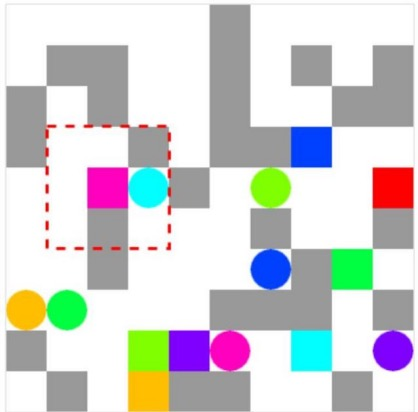
\includegraphics[width=0.75\columnwidth]{grid-environment}
\caption{A $10\!\times\!10$ grid world with 30\% obstacle density
and 8 robots.
Colored squares indicate start positions; colored circles indicate
goals; gray circles represent obstacles; the red dashed box shows
the $3\!\times\!3$ FOV.}
\label{fig:grid_env}
\end{figure}

\textbf{Scalability evaluation.}
To further verify generalization across different robot counts,
the model trained with 8 robots is tested with 16, 32, 64, and
128 robots.
Fig.~\ref{fig:scalability} shows that while success rate decreases
as the number of robots increases, \rmha{} maintains high success
rates from 16 to 64 robots and avoids performance collapse at 128
robots, demonstrating good scalability.

\begin{figure}[t]
\centering
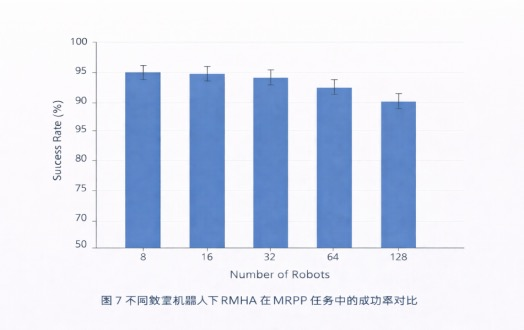
\includegraphics[width=0.85\columnwidth]{scalability}
\caption{Success rate of \rmha{} under different robot counts.}
\label{fig:scalability}
\end{figure}

All experiments are conducted on an Ubuntu server with dual NVIDIA
RTX 8000 GPUs, using PyTorch~2.1 and Python~3.7.

% ── 3.2 Baselines and Metrics ──────────────────────────────
\subsection{Baselines and Evaluation Metrics}

\textbf{Baselines.}
We compare with three state-of-the-art MARL-based MRPP methods:
\textbf{SCRIMP}~\cite{wang2023scrimp} (GNN-based scalable
communication, FOV $3\!\times\!3$),
\textbf{DHC}~\cite{ma2021distributed} (GNN-based communication,
FOV $9\!\times\!9$), and
\textbf{PICO} (ad-hoc routing communication, FOV
$11\!\times\!11$).
We also include the classical centralized planner
\textbf{ODrM*}~\cite{ellis2021mapf} with inflation factor
$\epsilon\!=\!2.0$ and a 5-minute timeout.

\textbf{Metrics.}
\begin{itemize}
\item \textbf{Max Reached (MR):} the maximum number of robots
  that reach their goals at any time step.
\item \textbf{Collision Rate (CO):} the ratio of collision events
  (with obstacles or other robots) to the product of episode
  length and robot count.
\item \textbf{Success Rate (SR):} the percentage of episodes in
  which all robots reach their goals collision-free within the
  time limit $T_{\max}$:
  \begin{equation}\label{eq:sr}
    S_r = \frac{N_{\mathrm{success}}}{N_{\mathrm{total}}}
        \times 100\%.
  \end{equation}
  Statistical significance is ensured by running at least 100
  episodes per setting.
\end{itemize}

% ── 3.3 Results ─────────────────────────────────────────────
\subsection{Results and Analysis}

\subsubsection{Communication Ablation Study}

To evaluate the contribution of the Transformer-based
communication mechanism, we develop two ablation baselines:
\begin{itemize}
\item \textbf{MAPPO}: the communication module is entirely
  removed; robots never send or receive messages.
\item \textbf{MAPPO+Graph Comm}: attention weights are computed
  based on message content alone, without fusing Manhattan
  distance embeddings.
\end{itemize}
All experiments use 128 robots in a $40\!\times\!40$ grid at
obstacle densities of 0\%, 15\%, and 30\%.

\begin{figure}[t]
\centering
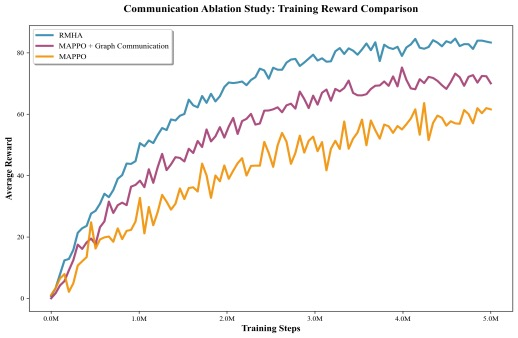
\includegraphics[width=\columnwidth]{ablation-reward}
\caption{Communication ablation: training reward curves.}
\label{fig:ablation_reward}
\end{figure}

Fig.~\ref{fig:ablation_reward} shows the training reward over
time.
All three methods exhibit rapid reward increase in the early
stages.
However, \rmha{} and MAPPO+Graph Comm converge faster and more
stably, while MAPPO rises more slowly with larger variance,
indicating the significant advantages of graph communication in
training efficiency and convergence.

\begin{figure}[t]
\centering
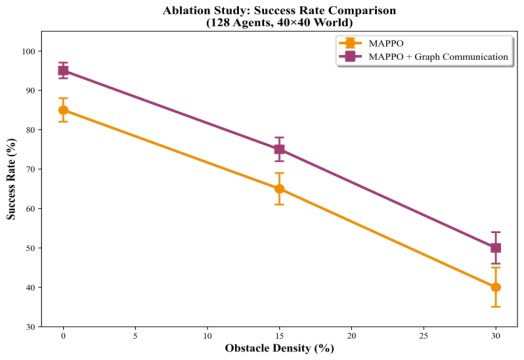
\includegraphics[width=0.85\columnwidth]{ablation-sr-mappo-vs-graphcomm}
\caption{Communication ablation: success rate comparison between
MAPPO and MAPPO+Graph Comm.}
\label{fig:ablation_sr1}
\end{figure}

\begin{figure}[t]
\centering
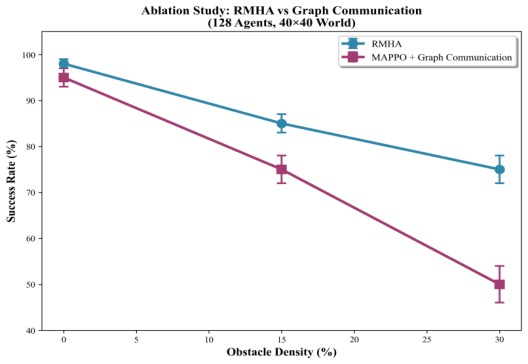
\includegraphics[width=0.85\columnwidth]{ablation-sr-rmha-vs-graphcomm}
\caption{Communication ablation: success rate comparison between
MAPPO+Graph Comm and \rmha.}
\label{fig:ablation_sr2}
\end{figure}

As shown in Figs.~\ref{fig:ablation_sr1}
and~\ref{fig:ablation_sr2}, the success rate of all methods
decreases with increasing obstacle density.
MAPPO+Graph Comm consistently outperforms MAPPO---at 30\% density,
MAPPO's success rate drops to approximately 40\% while Graph Comm
remains around 50\%, demonstrating that multi-head self-attention
communication helps robots perceive others' intentions and
positions.
\rmha{} further improves upon Graph Comm: at 30\% density,
\rmha{} achieves approximately 75\% success rate (vs.\ 50\% for
Graph Comm), confirming that Manhattan distance-based relation
encoding enables more accurate understanding of spatial
relationships and produces better decisions under complex, dynamic
conditions.

\begin{figure}[t]
\centering
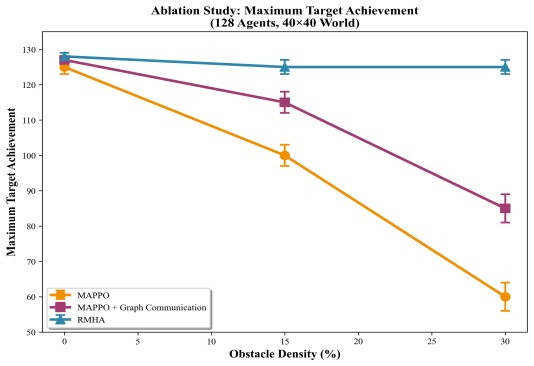
\includegraphics[width=0.85\columnwidth]{ablation-max-reached}
\caption{Communication ablation: maximum goals reached across
obstacle densities.}
\label{fig:ablation_mr}
\end{figure}

Fig.~\ref{fig:ablation_mr} shows the maximum goals reached.
MAPPO's performance drops rapidly with increasing density, while
\rmha{} maintains near 125 goals even in high-density
environments.
These results confirm that distance-relation enhancement
effectively fuses other robots' information in complex cooperative
tasks, improving both efficiency and robustness.

Overall, in the 128-robot, 30\%-density setting, the success rate
of \rmha{} exceeds that of the non-enhanced communication method
by 53\%, verifying the algorithm's generalization capability and
robustness at scale.

% ── 3.3.2 Comparison with SOTA ─────────────────────────────
\subsubsection{Comparison with State-of-the-Art Methods}

To further evaluate \rmha, we compare it with ODrM*, SCRIMP,
DHC, and PICO on two types of benchmark maps: \textbf{Warehouse}
maps (regular shelf aisles and narrow corridors simulating
pick-and-place scenarios) and \textbf{City/Game} maps (irregular
block/maze-like layouts simulating urban traffic or game levels).
All experiments use a $40\!\times\!40$ grid with 128 robots.
For each map type and obstacle complexity level (0\%, 15\%, 30\%),
100 reproducible map instances are sampled with fixed random seeds;
all algorithms run on the same instances to ensure fairness.
Mean values with confidence intervals are reported.

\begin{figure}[t]
\centering
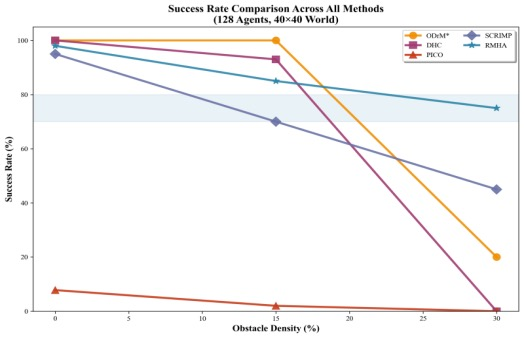
\includegraphics[width=\columnwidth]{comparison-sr}
\caption{Success rate comparison across algorithms on Warehouse
and City/Game maps.}
\label{fig:comp_sr}
\end{figure}

As shown in Fig.~\ref{fig:comp_sr}, all algorithms' success rates
decline with increasing obstacle complexity.
At low complexity (0\%), \rmha{} performs comparably to ODrM* and
SCRIMP.
As complexity increases to 15\% and 30\%, \rmha's advantage
becomes progressively larger.
At 30\%, \rmha{} maintains a success rate of approximately 75\%,
while SCRIMP falls below 50\%, ODrM* drops to roughly 20\% (within
the 5-minute planning limit), and DHC and PICO exhibit severe
performance degradation.

\begin{figure}[t]
\centering
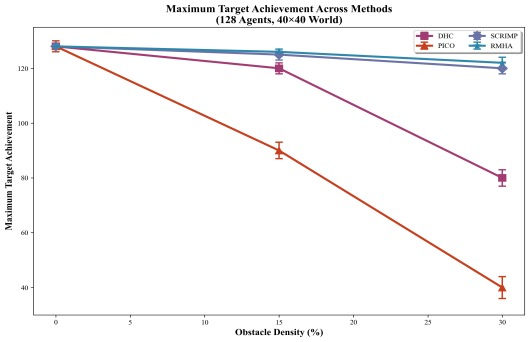
\includegraphics[width=\columnwidth]{comparison-max-reached}
\caption{Maximum goals reached across algorithms on Warehouse
and City/Game maps.}
\label{fig:comp_mr}
\end{figure}

Fig.~\ref{fig:comp_mr} shows the maximum goals reached.
PICO and DHC degrade fastest despite having communication
mechanisms, as they lack effective modeling of dynamic inter-robot
relationships.
In contrast, SCRIMP and \rmha, which employ graph
attention/Transformer-based communication, maintain 120+~goals
even at 30\% density.
\rmha{} further benefits from spatial relation encoding, enabling
more precise modeling of interaction intensity and local congestion
structure, thus improving both interpretability and robustness.

% ── 3.3.3 Trajectory Visualization ─────────────────────────
\subsubsection{Trajectory Visualization}

Fig.~\ref{fig:trajectory} compares the global trajectories of
\rmha{} and MAPPO in a complex environment.
\rmha{} produces well-organized trajectories with fewer path
conflicts, whereas MAPPO exhibits significant crossing and
clustering in local areas, with some robots stalling for extended
periods.

\begin{figure}[t]
\centering
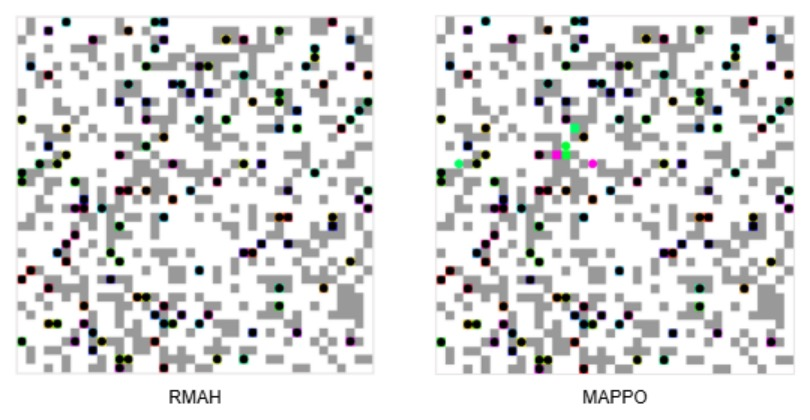
\includegraphics[width=\columnwidth]{trajectory-comparison}
\caption{Global trajectory comparison: \rmha{} (left) vs.\
MAPPO (right).}
\label{fig:trajectory}
\end{figure}

\begin{figure}[t]
\centering
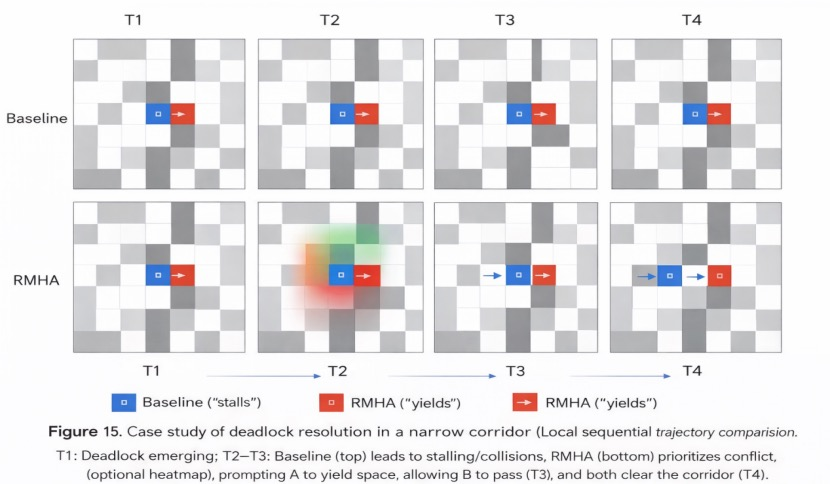
\includegraphics[width=\columnwidth]{deadlock-resolution}
\caption{Deadlock resolution in a narrow corridor.
At $T_1$, robots A and B enter a conflict;
the baseline leads to deadlock by $T_2$--$T_3$.
Under \rmha, robot~A yields at $T_3$, allowing B to pass, and
both proceed by $T_4$.}
\label{fig:deadlock}
\end{figure}

To analyze fine-grained interaction behavior,
Fig.~\ref{fig:deadlock} shows a representative head-on encounter
in a narrow corridor ($10\!\times\!10$ crop).
Under the baseline, both robots adopt similar forward/wait
strategies, resulting in persistent deadlock.
Under \rmha, the spatial relation-enhanced attention mechanism
enables robot~A to perceive the proximity of the conflicting
neighbor, increase its attention weight on that relationship, and
proactively yield by taking a backward or lateral step, thereby
resolving the deadlock within two time steps.

These results demonstrate that \rmha{} not only improves overall
success rates but also effectively reduces deadlock probability in
high-conflict structures such as narrow corridors.

% ============================================================
%  4  CONCLUSION
% ============================================================
\section{Conclusion}

This paper investigated the cooperative communication problem in
multi-robot path planning from the perspectives of communication
mechanism modeling, algorithmic framework integration, and
experimental validation.
We proposed \rmha, a spatial relation-enhanced multi-head attention
communication method based on graph attention mechanisms.
By incorporating relative distance information between robots into
the attention weight computation, \rmha{} dynamically adjusts
communication weights, significantly reducing communication
overhead while improving path planning success rates.

Experiments demonstrate that \rmha{} exhibits high adaptability
and robustness across varying obstacle densities, with
particularly strong performance in high-density scenarios where
its success rate substantially exceeds existing methods.
Communication ablation studies further confirm the critical role of
inter-robot distance information in optimizing path planning
decisions.

In summary, \rmha{} provides an effective solution for efficient
cooperation in complex multi-robot environments, offering a new
perspective on intelligent agent communication and collaboration.

% ============================================================
%  REFERENCES
% ============================================================
\bibliographystyle{IEEEtran}
\begin{thebibliography}{31}

\bibitem{wang2023scrimp}
Y.~Wang, B.~Ang, S.~Huang, \etal,
``SCRIMP: Scalable communication for reinforcement- and
imitation-learning-based multi-agent pathfinding,''
in \emph{Proc. IEEE/RSJ Int. Conf. Intell. Robots Syst. (IROS)},
2023, pp.~9301--9308.

\bibitem{li2021lifelong}
J.~Li, A.~Tinka, S.~Kiesel, \etal,
``Lifelong multi-agent path finding in large-scale warehouses,''
in \emph{Proc. AAAI Conf. Artif. Intell.}, vol.~35, no.~13,
2021, pp.~11272--11281.

\bibitem{zhang2023warehouse}
Y.~Zhang, M.~C. Fontaine, V.~Bhatt, \etal,
``Multi-robot coordination and layout design for automated
warehousing,''
\emph{arXiv preprint arXiv:2305.06436}, 2023.

\bibitem{dresner2008multiagent}
K.~Dresner and P.~Stone,
``A multiagent approach to autonomous intersection management,''
\emph{J. Artif. Intell. Res.}, vol.~31, pp.~591--656, 2008.

\bibitem{ma2022graph}
H.~Ma,
``Graph-based multi-robot path finding and planning,''
\emph{Current Robot. Rep.}, vol.~3, no.~3, pp.~77--84, 2022.

\bibitem{tamura2025human}
H.~Tamura, T.~Konno, K.~Ito, \etal,
``Human behavior and comfort during load carrying to autonomous
mobile robot,''
\emph{Int. J. Social Robot.}, pp.~1--19, 2025.

\bibitem{silver2005cooperative}
D.~Silver,
``Cooperative pathfinding,''
in \emph{Proc. AAAI Conf. Artif. Intell. Interactive Digital
Entertainment}, vol.~1, 2005, pp.~117--122.

\bibitem{sharon2015cbs}
G.~Sharon, R.~Stern, A.~Felner, and N.~R. Sturtevant,
``Conflict-based search for optimal multi-agent pathfinding,''
\emph{Artif. Intell.}, vol.~219, pp.~40--66, 2015.

\bibitem{ren2021subdimensional}
Z.~Ren, S.~Rathinam, and H.~Choset,
``Subdimensional expansion for multi-objective multi-agent path
finding,''
\emph{IEEE Robot. Autom. Lett.}, vol.~6, no.~4,
pp.~7153--7160, 2021.

\bibitem{ellis2021mapf}
J.~Ellis,
``Multi-agent path finding with reinforcement learning,''
M.S. thesis, Stellenbosch Univ., Stellenbosch, 2021.

\bibitem{huang2021strategic}
L.~Huang and Q.~Zhu,
``The strategic value of observable cost in stochastic games,''
\emph{IEEE Trans. Cybern.}, vol.~52, no.~10,
pp.~10506--10519, 2021.

\bibitem{sartoretti2019primal}
G.~Sartoretti, J.~Kerr, Y.~Shi, \etal,
``Multi-agent path finding with prioritized communication
learning: Pathfinding via reinforcement and imitation multiagent
learning,''
\emph{IEEE Robot. Autom. Lett.}, vol.~4, no.~3,
pp.~2378--2385, 2019.

\bibitem{chung2024review}
J.~Chung, J.~Fayyad, Y.~A. Younes, \etal,
``Learning team-based navigation: A review of deep reinforcement
learning techniques for multi-agent pathfinding,''
\emph{Artif. Intell. Rev.}, vol.~57, no.~2, p.~41, 2024.

\bibitem{wang2025lns2rl}
Y.~Wang \etal,
``LNS2+RL: Combining multi-agent reinforcement learning with
large neighborhood search in multi-agent path finding,''
in \emph{Proc. AAAI Conf. Artif. Intell.}, vol.~39, no.~22,
2025.

\bibitem{li2020gnn}
Q.~Li, F.~Gama, A.~Ribeiro, and A.~Prorok,
``Graph neural networks for decentralized multi-robot path
planning,''
in \emph{Proc. IEEE/RSJ Int. Conf. Intell. Robots Syst. (IROS)},
2020, pp.~11785--11792.

\bibitem{li2021magat}
Q.~Li, W.~Lin, Z.~Liu, and A.~Prorok,
``Message-aware graph attention networks for large-scale
multi-robot path planning,''
\emph{IEEE Robot. Autom. Lett.}, vol.~6, no.~3,
pp.~5533--5540, 2021.

\bibitem{ma2021distributed}
Z.~Ma, Y.~Luo, and H.~Ma,
``Distributed heuristic multi-agent path finding with
communication,''
in \emph{Proc. IEEE Int. Conf. Robot. Autom. (ICRA)},
2021, pp.~8699--8705.

\bibitem{guan2022abmapper}
H.~Guan, Y.~Gao, M.~Zhao, Y.~Yang, F.~Deng, and T.~L. Lam,
``Ab-mapper: Attention and BicNet based multi-agent path planning
for dynamic environment,''
in \emph{Proc. IEEE/RSJ Int. Conf. Intell. Robots Syst. (IROS)},
2022, pp.~13799--13806.

\bibitem{wang2025transformer}
P.~Wang, M.~Ghergherehchi, and J.~Kim,
``Transformer-based path planning for single-arm and dual-arm
robots in dynamic environments,''
\emph{Int. J. Adv. Manuf. Technol.}, vol.~139, no.~7--8,
pp.~1--19, 2025.

\bibitem{xiong2025ropt}
Z.~Xiong, Y.~Wang, and Y.~Tian \etal,
``RoPT: Route-planning model with Transformer,''
\emph{Appl. Sci.}, vol.~15, no.~9, pp.~4914, 2025.

\bibitem{lee2024mission}
K.~Lee, E.~Im, and K.~Cho,
``Mission-conditioned path planning with Transformer variational
autoencoder,''
\emph{Electronics}, vol.~13, no.~13, pp.~2437, 2024.

\bibitem{aina2025mlp}
S.~T. Aina and A.~B. Iyaomolere,
``Multi hand gesture recognition using a multilayer perceptron
(MLP) model with mmWave radar sensing data,''
\emph{J. Eng. Res. Rep.}, vol.~27, no.~11, pp.~194--203, 2025.

\bibitem{wang2025mlp}
X.~Wang, F.~Xu, and M.~Zhang,
``A transfer learning-enhanced multilayer perceptron for buffeting
response prediction of long-span bridges,''
\emph{J. Wind Eng. Ind. Aerodyn.}, vol.~267, p.~106258, 2025.

\bibitem{ouaret2025mlp}
A.~Ouaret, I.~S. Talantikite, H.~Lehouche, \etal,
``A direct adaptive control architecture for buildings thermal
comfort and energy efficiency optimization using multilayer
perceptron neural networks and model reference learning,''
\emph{Energy Build.}, vol.~349, p.~116528, 2025.

\bibitem{xiao2025collaborative}
H.~Xiao, L.~Fu, C.~Shang, \etal,
``Collaborative energy-saving path planning of unmanned surface
vehicle cluster based on multi-head attention mechanism and
multi-agent deep reinforcement learning,''
\emph{Eng. Appl. Artif. Intell.}, vol.~161, p.~112078, 2025.

\bibitem{chen2025predicting}
Z.~Chen, Y.~Liu, W.~Ni, \etal,
``Predicting driving comfort in autonomous vehicles using road
information and multi-head attention models,''
\emph{Nat. Commun.}, vol.~16, no.~1, p.~2709, 2025.

\bibitem{chen2023transportation}
S.~Chen and Y.~Liu,
``Research on transportation mode recognition based on multi-head
attention temporal convolutional network,''
\emph{Sensors}, vol.~23, no.~7, 2023.

\bibitem{zhou2025mappo}
Y.~Zhou, Y.~Yue, and B.~Yan \etal,
``Collaborative target tracking algorithm for multi-agent based
on MAPPO and BCTD,''
\emph{Drones}, vol.~9, no.~8, p.~521, 2025.

\bibitem{zhang2025mappo}
P.~Zhang and G.~Li,
``A cooperative dynamic target search approach for multi-UAV
systems utilizing the MAPPO algorithm,''
\emph{Discover Artif. Intell.}, vol.~5, no.~1, p.~153, 2025.

\bibitem{ding2025mappo}
Z.~Ding, X.~Wang, C.~Cai, \etal,
``Multi-UAV intelligent decision-making method with layer delay
dual-center MAPPO for air combat,''
\emph{Appl. Intell.}, vol.~55, no.~11, p.~811, 2025.

\end{thebibliography}

\end{document}
